\documentclass[12pt, times]{article}
\usepackage{booktabs}
\usepackage{makecell}
\usepackage{multirow}
\usepackage{fullpage}
\usepackage{csvsimple}
\usepackage{setspace}
\usepackage{graphicx}

\title{FIN9013 Assignment 1}
\author{Ang Zhang}

\begin{document}
\maketitle

\onehalfspacing

\section*{Introduction}
This report examines the determinants of the debt ratio of firms using a panel data of 16,257 observations.
The data management step processed the data by defining the dependent variable, $Debt$, as the total debt over total book asset.
The independent variables include the logarithm of annual sales turnover, $Size$, the market to book ratio of assets, $MB$,
and a dummy variable indicating whether the firm has R\&D spending, $D(RD)$.
Varies models, including linear models and discrete choice models are used to examine the relationshio.
To account for the potential endogeneity of the MB variable, instrument variables is introduced and
validated through two stage LS. Then, panel data estimation is performed to account for
heterogeneity (potential correlation between the error terms across firms/years).

Moving on, treatment effect is studied with DD analysis to examine a shock to a subset of the firms 
located in a specific region. Matching model is also used to estimate the treatment effect which shows similar results.

The report is organized as follows: Table 1 in appendix presents summary statistics for the variables used in the analysis.
Each section presents the results of the different models used in the analysis, with detailed results
presented in tables in the appendix.

\section*{Linear regression, interactions, split-samples and non-linearities}

In the baseline model, the slope term of $Size$ factor is 0.0237, 
which means that for a one unit increase in the logarithm of annual sales turnover, 
measured in millions, the predicted value of the debt ratio, measured by the total debt over total book asset, \
increase by 0.0237, holding all other variables constant.
The slope term of $MB$ factor is 0.0085, which means that for a one unit increase in the market to book ratio of assets, 
the predicted value of the debt ratio, measured by the total debt over total book asset, \
increase by 0.0.0085, holding all other variables constant.
The slope term of $D(RD)$ factor is -0.0902, which means that for a firm with positive R\&D spending, 
the predicted value of the debt ratio, measured by the total debt over total book asset, \
is 0.0902 lower than a comparable firm with no R\&D spending, holding all other variables constant.
\newline
However, we can hardly say that this model is a good fit, as the $R^2$ value is only 0.0813, which means that only 8.13\% of the
variation in the dependent variable, $Debt$, can be explained by the independent variables, $Size$, $MB$ and $D(RD)$,
while the rest 91.87\% of the variation is due to other factors not included in the model.
\newline
When all variables are held at their mean, the predicted value of $Debt$ is 0.2029, while for all variables at their 
median the predicted $Debt$ value is 0.1655.
\newline
The effect of $D(RD)$ on $Debt$ is constant and always at $\beta_{rd}$, no matter where MB stands at.
That's because in eq.(1), there's no interaction term so the coefficient of $D(RD)$ which is $\beta_{rd}$ solely determines the effect
that $D(RD)$ has on $Debt$.
\newline
Comparing the coefficient of $MB$ in the RD Model and the No RD Model, 
we can see that the coefficient of $MB$ in the RD Model is 0.0015, while 
in the No RD Model it is -0.0173. This suggests that the effect of $MB$ have different
effects on the debt ratio for firms with and without R\&D spending. 
\newline
Comparing the two models where RD *rank* is included as rank in one of them (RD Rank Model)
and RD *rank* is included as class in the other one (RD Class Model), we can see that the parameter
estimates for the four categorical variables are quite different. Also, the
 RD Rank Model has a higher $R^2$ value, which means that it explains more of the 
 variation in the dependent variable. This suggests that the effect of R\&D spending
 might is likely non-linear, and that the RD Rank Model is a better fit for the data.

\section*{Discrete choice variables and censoring}

The Python statsmodel package does not support the estimation of a Tobit model, so I manually defined a class to estimate the Tobit model.
The model class inherits from the statsmodel GLM class, and the log-likelihood function is defined as the sum of the log-likelihood of the
censored and uncensored observations. 
The discrete choice model built-in the statsmodel package do offer a marginal effect function (get\_margeff) to calculate the
marginal effect of the independent variables. But the question with this package is that it cannot account for interaction terms.
The reason is that in statsmodel package, the model takes each interaction term as a separate variable, so the marginal effect
function cannot calculate the marginal effect of the interaction term. But for logit model, the marginal effect can be calculated
manually by taking the derivative of the probability function with respect to the independent variable and there's a closed-form solution as below:
\begin{equation}
    \frac{\partial P(Debt|D(RD))}{\partial D(RD)} = (\beta_{rd} + \beta_{mbrd} MB ) \cdot P(y=1|x) \cdot (1-P(y=1|x))
\end{equation}
where $P(y=1|x)$ is the estimated logic probability, at the point where the marginal effect is to be calculated. 


\section*{Instrumental variables}
For an instrument to be valid, it must be correlated with the endogenous variable, $MB$, 
but uncorrelated with the error term. The first assumption is tested by regressing $MB$ on the instrument and look at the statistics
including R-squared and F-statistics. But the second assumption cannot be tested directly, because the endogenous variable 
have distorted the error term so that the error term is no longer a "real" error term.
But we can use economecal intuition to think about whether the instrument is likely to be correlated with the error term.
Heuristically, which month did the firm go public is unlikely to be correlated with the debt ratio, because the month of the IPO
is unlikely to have any effect on the how much debt the firm decides to take on.
But a firm that goes public in December may face significantly different market conditions
when many investors are on vacation, thus may experience a dip in their valuation, thus negatively impacting
their market value. Even though market condition would revert, the initial market perception of the firm
would continue to be at play and exibits a path dependence which persistently play a part in the firms's market value.

\section*{Panel data estimation}
The agumented model with \textit{D(DecIPO)} shows insiginificant coefficient for this added dummy variable.
That is expected because the IPO month of a firm is either in December or not in December, so 
this dummy variable is absorbed by the fixed effects of the firm.

\section*{DD analysis}
The baseline model shows a positive coefficient for \textit{D(Post)} and a negative coefficient for 
\textit{D(Treated)}, while controlling for Size, MB, and D(RD). With firm fixed effects, the variable \textit{D(Treated)} is fully
absorbed because a firm is either in NY/CA or not, unless the firm has moved either from NY/CA to other states or
from other states to NY/CA. With both firm fixed effects and year fixed effects, both \textit{D(Treated)} and \textit{D(Post)} are absorbed
because again, \textit{D(Treated)} only depends on the year which is absorbed into year FE. In all three models, the interaction
term between \textit{D(Treated)} and \textit{D(Post)} is insignificant.
When examining the set of indicators for each year together with \textit{D(Treated)}, a clear trend can be spotted. 
Recall that key identifying assumption of DD is “Parallel Trends”, which stipulates that no correlation between outcome 
and assignment, and that in absence of treatment, the outcome for treated and controls is unaffected.
From Figure \ref{fig:parallel_trends}, we can see that the trend of the debt ratio for the treated group and the control group
is parallel before the treatment, which is the year 2000. After the treatment, the debt ratio for the treated group increases more than the trend
suggested by the control group. This suggests that the treatment has a positive effect on the debt ratio of the treated group.
This is also consistent with the coefficients in the baseline model.

\begin{figure}[h!]
    \centering
    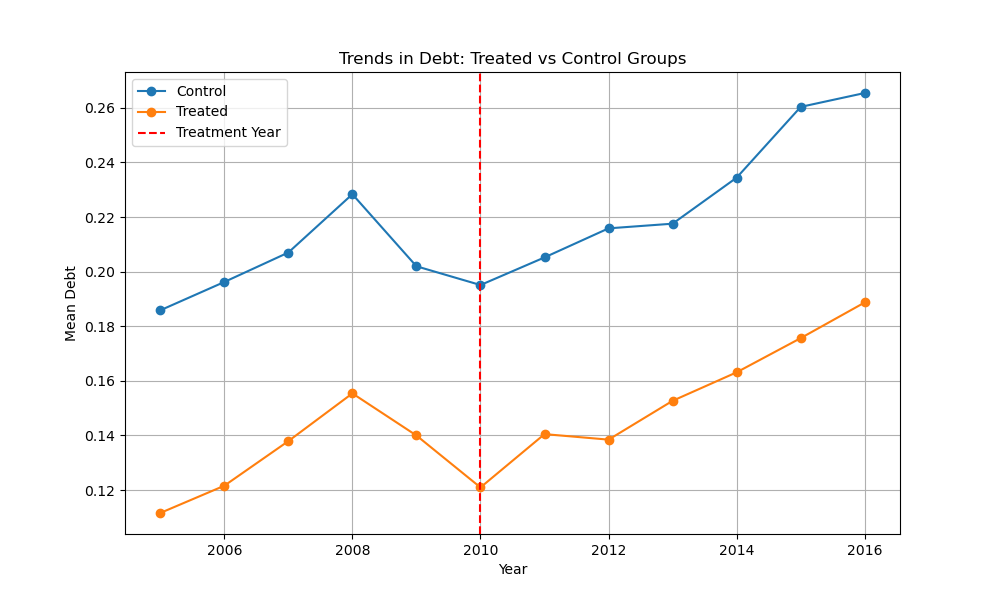
\includegraphics[width=0.8\textwidth]{parallel_trends.png}
    \caption{Parallel Trends Assumption}
    \label{fig:parallel_trends}
\end{figure}

\section*{Matching models}
In year 2010 only, the coefficient of \textit{D(Treated)} is -0.049 and significant at 5\% level, which (may) suggest that
firms in NY/CA that are affected by the shock have a lower debt ratio than firms in other states. This is consistent with the DD analysis.
With propensity score matching, the coefficient of \textit{D(Treated)} is -0.039 and significant at 5\% level.
This suggests that the treatment effect is robust. The implication of the matching model is that for firm with close probability
of receiving treatment based on their \textit{Size}, \textit{MB}, and \textit{D(RD)}, the treated firm exhibits a lower debt ratio
than their "matches" in other states. This is consistent with the DD analysis and the baseline model.
Using a nearest neighbor matching of 2 neighors give a similar result, with the coefficience of \textit{D(Treated)} of -0.043
and again significant at 5\% level. This suggests that the treatment effect is robust to the choice of the number of neighbors.

\section*{Appendix}

\begin{table}[h!]
    \centering
    \caption{Summary Statistics Table}
    \label{table:1}
    \begin{tabular}{lcccccccc}
        \toprule
        \multicolumn{8}{c}{Panel A: All Firms} \\
        \midrule
        Variable & N & Mean & StdDev & Min & P25 & Median & P75 & Max \\
        \midrule
        Debt & 16257 & 0.197 & 0.225 & 0 & 0.000 & 0.129 & 0.317 & 1.017 \\
        Size & 16257 & 5.786 & 2.060 & -0.997 & 4.576 & 5.991 & 7.194 & 10.068 \\
        MB & 16257 & 1.912 & 1.549 & 0.334 & 0.923 & 1.397 & 2.344 & 8.834 \\
        D\_RD & 16257 & 0.582 & 0.493 & 0 & 0 & 1.000 & 1.000 & 1.000 \\
        RD\_rank & 16257 & 1.908 & 1.120 & 1.000 & 1.000 & 2.000 & 2.000 & 5.000 \\
        D\_Debt & 16257 & 0.336 & 0.472 & 0 & 0 & 0 & 1.000 & 1.000 \\
        D\_DecIPO & 16257 & 0.089 & 0.285 & 0 & 0 & 0 & 0 & 1.000 \\
        \midrule
        \multicolumn{8}{c}{Panel B: Firms with R\&D} \\
        \midrule
        Variable & N & Mean & StdDev & Min & P25 & Median & P75 & Max \\
        \midrule
        Debt & 9468 & 0.150 & 0.201 & 0 & 0 & 0.058 & 0.246 & 1.017 \\
        Size & 9468 & 5.183 & 2.168 & -0.997 & 3.908 & 5.299 & 6.658 & 10.068 \\
        MB & 9468 & 2.202 & 1.699 & 0.334 & 1.064 & 1.644 & 2.760 & 8.834 \\
        D\_RD & 9468 & 1.000 & 0 & 1.000 & 1.000 & 1.000 & 1.000 & 1.000 \\
        RD\_rank & 9468 & 2.559 & 1.068 & 2.000 & 2.000 & 2.000 & 3.000 & 5.000 \\
        D\_Debt & 9468 & 0.245 & 0.430 & 0 & 0 & 0 & 0 & 1.000 \\
        D\_DecIPO & 9468 & 0.079 & 0.270 & 0 & 0 & 0 & 0 & 1.000 \\
        \midrule
        \multicolumn{8}{c}{Panel C: Firms without R\&D} \\
        \midrule
        Variable & N & Mean & StdDev & Min & P25 & Median & P75 & Max \\
        \midrule
        Debt & 6789 & 0.264 & 0.239 & 0 & 0.049 & 0.226 & 0.401 & 1.017 \\
        Size & 6789 & 6.626 & 1.548 & -0.997 & 5.686 & 6.647 & 7.689 & 10.068 \\
        MB & 6789 & 1.508 & 1.199 & 0.334 & 0.807 & 1.140 & 1.748 & 8.834 \\
        D\_RD & 6789 & 0 & 0 & 0 & 0 & 0 & 0 & 0 \\
        RD\_rank & 6789 & 1.000 & 0 & 1.000 & 1.000 & 1.000 & 1.000 & 1.000 \\
        D\_Debt & 6789 & 0.463 & 0.499 & 0 & 0 & 0 & 1.000 & 1.000 \\
        D\_DecIPO & 6789 & 0.103 & 0.304 & 0 & 0 & 0 & 0 & 1.000 \\
        \bottomrule
    \end{tabular}
    \newline
    \textit{Note: This table presents the summary statistics for the variables used in the analysis. Panel A includes all firms, Panel B includes firms with R\&D, and Panel C includes firms without R\&D.}
\end{table}

\begin{table}[h!]
    \centering
    \caption{Parameter Estimates of Each Model}
    \label{table:2}
    \begin{tabular}{lccccccc}
        \toprule
        Parameter & \makecell{Model \\ Baseline} & \makecell{Model \\ Interaction} & \makecell{Model \\ Augmented} & \makecell{Model \\ RD} & \makecell{Model \\ No RD} & \makecell{Model \\ RD Rank} & \makecell{Model \\ RD Class} \\
        \midrule
        Intercept & \makecell{0.1114*** \\ (0.0068)} & \makecell{0.1298*** \\ (0.0072)} & \makecell{0.1029*** \\ (0.0119)} & \makecell{0.0292*** \\ (0.0063)} & \makecell{0.1029*** \\ (0.0131)} & \makecell{0.0376*** \\ (0.0090)} & \makecell{0.1070*** \\ (0.0071)} \\
        Size & \makecell{0.0237*** \\ (0.0009)} & \makecell{0.0242*** \\ (0.0009)} & \makecell{0.0282*** \\ (0.0017)} & \makecell{0.0227*** \\ (0.0009)} & \makecell{0.0282*** \\ (0.0018)} & \makecell{0.0297*** \\ (0.0010)} & \makecell{0.0334*** \\ (0.0010)} \\
        MB & \makecell{-0.0033*** \\ (0.0011)} & \makecell{-0.0175*** \\ (0.0022)} & \makecell{-0.0173*** \\ (0.0022)} & \makecell{0.0015 \\ (0.0012)} & \makecell{-0.0173*** \\ (0.0024)} & \makecell{-0.0072*** \\ (0.0012)} & \makecell{-0.0067*** \\ (0.0011)} \\
        D\_RD & \makecell{-0.0771*** \\ (0.0037)} & \makecell{-0.1092*** \\ (0.0055)} & \makecell{-0.0737*** \\ (0.0137)} & & & \\
        MB*D\_RD & & \makecell{0.0194*** \\ (0.0025)} & \makecell{0.0188*** \\ (0.0025)} & & & \\
        Size*D\_RD & & & \makecell{-0.0055*** \\ (0.0020)} & & & \\
        RD\_rank & & & & & &\makecell{0.0008 \\ (0.0020)} &  \\
        RD\_rank 1 & & & & & & & \makecell{-0.0547*** \\ (0.0081)} \\
        RD\_rank 2 & & & & & & & \makecell{-0.1358*** \\ (0.0076)} \\
        RD\_rank 3 & & & & & & & \makecell{-0.1473*** \\ (0.0097)} \\
        RD\_rank 4 & & & & & & & \makecell{-0.0337** \\ (0.0158)} \\
        \midrule
        RSquare & 0.1054 & 0.1086 & 0.1091 & 0.0586 & 0.0419 & 0.0809 & 0.1253 \\
        \#Obs & 16257 & 16257 & 16257 & 9468 & 6789 & 16257 & 16257 \\
        \bottomrule
    \end{tabular}
    \newline
    \textit{Note: This table presents the parameter estimates for various models. 
    The baseline model includes the intercept, Size, and MB. 
    The interaction model adds an interaction term between MB and D\_RD. 
    The augmented model includes additional interaction terms. 
    The RD model includes only firms with R\&D, while the No RD model includes firms without R\&D. 
    The RD Rank model includes the RD\_rank variable, 
    and the RD Class model includes categorical variables for RD\_rank. 
    Standard errors are in parentheses. 
    Significance levels are indicated by * p<0.1, ** p<0.05, *** p<0.01.}
\end{table}

\end{document}